\chapter{Etat de l'art}
\label{sec:etat de l'art}

\section*{Introduction}

Pour mettre en place l’application KOOPT, il était nécessaire d’utiliser un large spectre de notions et de technologies. KOOPT a été développé sous Android Studio en utilisant différents outils Android, ainsi que KOOPT utilise des Web Services (REST), ainsi que Crashlytics Fabric et les Logs pour faciliter le débogage de l’application.
\addcontentsline{toc}{section}{Introduction.}



\section{L’environnement logiciel}
\subsection{Android}
\subsubsection{Présentation d’android}
Android est la plate-forme mobile la plus populaire au monde.Avec des centaines de millions d'appareils mobiles dans plus de 190 pays à travers le monde Android est la plus grande base installée de toute plate-forme mobile, chaque jour un million d’utilisateurs Android découvre cette plateforme pour la première fois et commence à chercher des applications, des jeux et d'autres contenus numériques.
Android donne une plate-forme open source de classe mondiale pour créer des applications et des jeux pour les utilisateurs Android partout, ainsi qu'un marché ouvert pour les distribuer instantanément.

\subsubsection{Architecture d’Android}


Comme le montre le schéma ci-dessous, la plateforme Android est basée sur 5 couches :
- un noyau linux.  qui fournit les drivers nécessaires 
- un ensemble d’API C/C++ fournissant des fonctionnalités de plus haut niveau (SQLite, OpenGL ES 2.0…)
- un framework java exploitable par toutes les applications s’exécutant sur la machine virtuelle Dalvik
- un ensemble d’application déjà fourni couvrant les besoins standards.
 
\begin{figure}[H]
\begin{center}
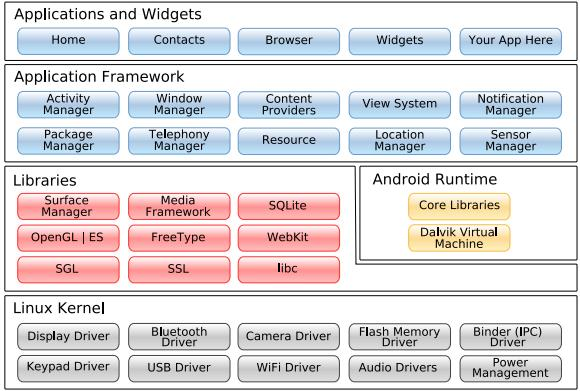
\includegraphics[width=1\linewidth]{images/architecture_android}
\end{center}
\caption{L'architecture de l'Android}
\label{fig:1}
\end{figure}

\subsubsection{L’IDE Android studio}


Android Studio est l’environnement de développement des applications Android officiel de Google qui remplace l’IDE d’Eclipse (avec donc exactement les mêmes fonctionnalités) depuis le 8 décembre 2014, il est basé sur  IntelliJ IDEA. 
Android Studio permet principalement d'éditer les fichiers Java et les fichiers de configuration d'une application Android.

Il propose entre autres des outils pour gérer le développement d'applications multilingues et permet de visualiser la mise en page des écrans sur des écrans de résolutions variées simultanément.
En plus d’être un éditeur de code très puissant, Android Studio offre encore plus de fonctionnalités qui améliorent la productivité des applications Android, tels que :

- Un système de building des applications souple basé sur Gradle.

- Un émulateur rapide et riche en fonctionnalités.

- Un environnement unifié où le développeur peut développer pour tous les appareils
Android.

- L’exécution instantanée (Instant Run) pour apporter des modifications à une appli-
cation en cours d’exécution sans avoir à reconstruire un nouveau APK.

- Modèles de code et une intégration sur GitHub pour construire des fonctionnalités
communes d’applications.

- Des outils et frameworks de tests extensifs.
 
\textbf{Gradle:}


Gradle est un moteur de production qui fonctionne sur la plateforme Java, il est le digne successeur de Maven et de Ant, alliant ces deux outils afin de créer une plateforme de production Java simple à utiliser, et bien adaptée pour les projets Android.
Gradle est intégré à Android Studio et est utilisé afin de gérer et construire les projets Android (en utilisant le langage Groovy).
Il permet entre-autre de gérer la construction d’un projet utilisant plusieurs modules et dépendances de librairies Maven, et ce, de façon très simple.\cite{gradle} 



\subsection{Quelques outils Android utilisés}
\subsubsection{Adapter}

Adapter est un objet permettant de stocker des données provenant des différents sources (contact, rendrez-vous, ...) afin de pouvoir les afficher dans des composants  UI.
les adapters sont donc des interfaces entre les sources de  données et les IHM. 

L'adapter n'est en fait qu'une interface qui définit les comportements généraux des adaptateurs. Cependant, la construction d'un adaptateur, nécessite la dérivation de BaseAdapter.

\begin{figure}[H]
\begin{center}
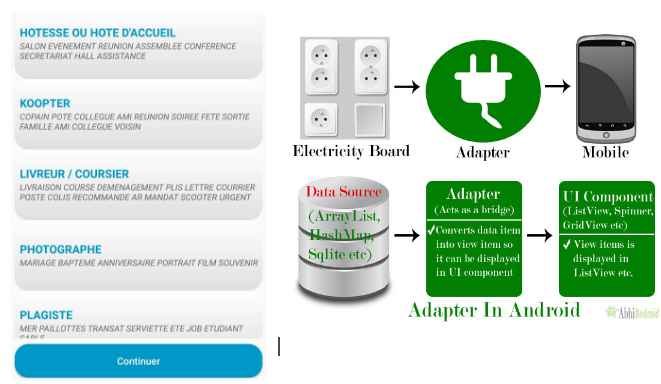
\includegraphics[width=1\linewidth]{images/adapter}
\end{center}
\caption{L'adapter dans l'Android}
\label{fig:2}
\end{figure}


\subsubsection{AsyncTask}


L’AsyncTask permet de réaliser des tâches de manière asynchrone, à la manière de la classe Thread. L’avantage de l’AsyncTask est sa simplicité d’utilisation et d’implémentation. Le Thread secondaire est créé automatiquement et la communication entre les différents Thread est simplifiée.
AsyncTask doit être hérité par la classe qui a été  créé, cette classe doit impérativement implémenter une méthode (doInBackground(Params...)),
Quand un AsynckTask s'exécute il passe par trois étape 


onPreExecute(), appelé sur le thread d’interface avant que la tâche soit exécutée. Cette étape est normalement utilisée pour configurer la tâche, par exemple, en montrant une barre de progression dans l’interface utilisateur.


doInBackground(Params...), invoqué sur le thread en arrière-plan immédiatement après OnPreExecute (). Cette étape est utilisée pour effectuer le calcul de fond qui peut prendre un certain temps. Les paramètres de la tâche asynchrone sont passés à cette étape. Le résultat du calcul doit être retourné par cette étape et sera renvoyé à la dernière étape. Cette étape peut également utiliser publishProgress (Progress …) de publier une ou plusieurs unités de progression. Ces valeurs sont publiées sur le thread d’interface utilisateur, à l’étape onProgressUpdate (Progress …).


onProgressUpdate(Progress...), invoqué sur le thread d’interface utilisateur après un appel à publishProgress (Progress …). Le moment de l’exécution est indéfini. Cette méthode est utilisée pour afficher toute forme de progression dans l’interface utilisateur tandis que le calcul de fond est toujours en cours d’exécution. Par exemple, il peut être utilisé pour animer une barre de progression ou afficher des logs.


onPostExecute(Result), appelé sur le thread UI après la fin du calcul. Le résultat est transmis à cette étape en tant que paramètre.
 
Pour que cette classe fonctionne correctement, il y a quelques règles à respecter :


\begin{itemize}
    \item La classe AsyncTask doit être chargée sur le thread UI. Ceci est fait automatiquement.
    \item L’instance de la tâche doit être créée sur le thread UI.
    \item execute(Param …) doit être invoqué sur le thread UI.
    \item Ne pas appeler OnPreExecute(), onPostExecute (Résultat), doInBackground(Param ...),  onProgressUpdate (Progress ...) manuellement.
    \item La tâche ne peut être exécutée qu’une seule fois (une exception sera levée si une deuxième exécution est tentée).
\end{itemize}\cite{asyncTask} 
 
\subsubsection{ContentProvider}


Un contentProvider sert à stocker et récupérer des données et ainsi les rendre accessibles à toutes les applications. C’est le moyen le plus connu de partager des données entres différentes applications. Par exemple, il existe un Content Provider gérant les Contacts d’un téléphone.
Android propose plusieurs ContentProviders basiques (audio, vidéo, images, informations sur les contacts…). Un contentProvider se compose d’une :

- Uri

- Méthodes (Insert, Update, Delete, Query).


Le chemin d’accès vers un ContentProvider se présente toujours sous forme d’une URI. Par exemple : 

content://com.example.transportationprovider/trains/122

  \textbf{A}      /          \textbf{B}            /    \textbf{C}  /  \textbf{D}  

\textbf{A} : Un préfixe standard, il sert à indiquer que les données sont contrôlées par un ContentProvider.
\newline
\textbf{B} : L’autorité qui contrôle cette URI. Elle identifie le ContentProvider responsable de cette URI. 
\newline
\textbf{C} : Permet au ContentProvider de savoir quelle donnée est requêtée par l’url. Ce segment est optionnel. Un content provider peut exposer plusieurs données (ici les trains) mais on pourrait avoir par exemple les voitures, donc ce ContentProvider pourra gérer deux types de données.
\newline
\textbf{D} : L’id de la donnée qu’on souhaite récupérer. (optionnel)


Pour créer un ContentProvider, il faut : 
    
- Mettre en place un système pour stocker les données (les contents providers utilisent généralement le SQLite).
    
- Étendre la classe ContentProvider.

- Déclarer le Content Provider dans le manifest (AndroidManifest.xml).\cite{provider} 


\subsubsection{SQLite}

 SQLite est une base de données open source, qui supporte les fonctionnalités standards des bases de données relationnelles comme la syntaxe SQL, les transactions et les PreparedStatement. La base de données nécessite peu de mémoire lors de l'exécution (env. 250 ko), ce qui en fait un bon candidat pour être intégré dans d'autres environnements d'exécution.
SQLite est intégrée dans chaque appareil Android. L'utilisation d'une base de données SQLite sous Android ne nécessite pas de configuration ou d'administration de la base de données. 
 
Il faut uniquement définir les instructions SQL pour créer et mettre à jour la base de données. Ensuite, celle-ci est gérée automatiquement, par la plate-forme Android. 
 
L'accès à une base de données SQLite implique l'accès au système de fichiers. Cela peut être lent. Par conséquent, il est recommandé d'effectuer les opérations de base de données de manière asynchrone. 
 
Si l’application crée une base de données, celle-ci est par défaut enregistrée dans le répertoire DATA /data/APP\_NAME/databases/FILENAME. 
 
Ce chemin de fichier est obtenu sur la base des règles suivantes : DATA est le chemin retourné par la méthode Environment.getDataDirectory(), APP\_NAME est le nom de l’application. FILENAME est le nom de la base de données qui est renseigné dans le code de votre application.\cite{sqlite}


\subsubsection{SharedPreferences}

Dans toutes applications, il est souvent nécessaire d'utiliser des variables qui doivent être gardées en mémoire même suite à une fermeture. La solution des Shared Preferences est la plus simple à implémenter.
Les SharedPreferences sont des espaces de stockages propres à chaque application Android. Avec un système de clé;valeur, vous pourrez persister vos données facilement.
Les SharedPreferences sont à récupérer depuis un context, avec context.getSharedPreferences(NAME,MODE).\cite{sharedpreference} 

\subsubsection{Les Logs}

 Comme chacun le sait, la méthode de débogage probablement la plus commune (quelque soit le langage), est d'utiliser des primitives d'affichage sur la sortie standard. Qui ne se rappelle pas des fameux printf du langage C ou des NSLog de l'Objective-C ? Le langage Java offre également la même possibilité grâce à des méthodes de type print du package System.out.
Le développement sur Android ne déroge pas à la règle puisque le SDK fournit une classe nommée android.util.Log qui inclue un bon nombre de méthodes d'aide au développement données dans la liste ci-dessous :\cite{log}

- Log.v : Affiche le message en mode “verbose” c'est à dire “verbeux” ou “abondant” en français.

- Log.d : Affiche le message en mode “debug”, utilisé pour le débuggage.

- Log.e : Affiche le message en mode “error” (erreur).

- Log.w : Affiche le message en mode “warning”, c'est à dire les avertissements.

- Log.i : Affiche le message en mode “info”.


\subsection{Méthodes et technologies déployées}

\subsubsection{Matériel design}

 Lors de la conférence Google I/O 2014, Google a dévoilé le design d'Android Lollipop, design qui portera le nom de Material Design. Ce design met l'accent sur l'unification de l'interface entre les différents types d'appareils : téléphones, tablettes, montres, télévisions mais touche aussi les sites web. De nombreux sites, dont ceux de Google, utilisent le Material Design qui est tout à fait adapté à la pratique du responsive. Pratique qui consiste à adapter l'interface aux dimensions de la fenêtre du navigateur.\cite{materiel}

Le Material Design est apparu quand le Flat Design commençait à faire parler de lui et Google a été rapidement clair sur le sujet : le Material Design n'est pas du Flat Design. Les plus sceptiques sur cette affirmation diront alors que c'est le Flat Design à la Google. Ils n'auront que partiellement raison. Même s'il est vrai que le Material Design partage un visuel similaire au Flat Design, il n'en dispose pas des principes forts du design fait par Google. Les designers de cette entreprise se sont mis au défi de créer un langage visuel pour leur utilisateurs qui se synthétisent en 3 grands principes.

Quelques composants graphiques utilisés dans KOOPT. 

\textbf{Le menu latéral:}
 

Le menu latéral est un composant lié à la navigation. Il se caractérise par un panneau latéral qui se déplace depuis l'extérieur de l'écran jusqu'à un certain niveau à l'intérieur. En général, il se place sur la gauche de l'écran mais il est possible de le placer à droite, voire d'en placer deux, un à gauche et un à droite de l'écran.




\begin{figure}[H]
\begin{center}
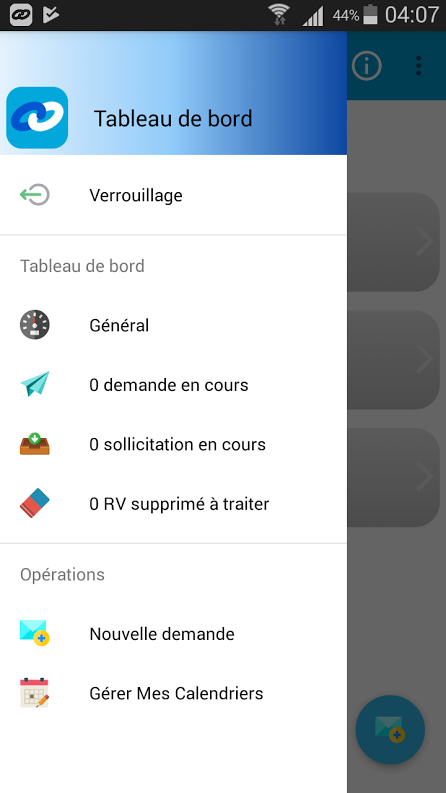
\includegraphics[width=0.5\linewidth]{images/menu_lateral}
\end{center}
\caption{Menu Latéral KOOPT}
\label{fig:3}
\end{figure}




\textbf{Les labels flottants:}
 
 
Ce composant permet à l'utilisateur de saisir du texte dans un espace dédié à cet effet. Par contre, donnez du sens à ce composant était fastidieux. Vous deviez créer un TextView au dessus pour lui donner un titre et y placez un hint.
la bibliothèque de design, nous permet spécifier un label flottant pour votre champ. Ce label se place dans le champ lorsque le curseur n'est pas dessus et se déplace en dehors lorsque vous y placez le curseur.

\begin{figure}[H]
\begin{center}
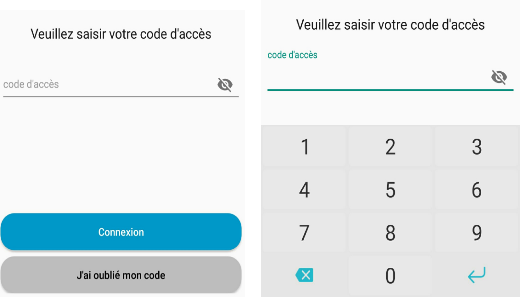
\includegraphics[width=1\linewidth]{images/label_flottant}
\end{center}
\caption{Label flottant KOOPT}
\label{fig:5}
\end{figure}

\subsubsection{Design pattern  Singleton}

KOOPT possède des classes qui doivent être instanciées une seule et unique fois pour cela elle utilise le design pattern Singleton.
le singleton est un patron de conception (design pattern) dont l'objectif est de restreindre l'instanciation d'une classe à un seul objet (ou bien à quelques objets seulement). Il est utilisé lorsqu'on a besoin exactement d'un objet pour coordonner des opérations dans un système. Le modèle est parfois utilisé pour son efficacité, lorsque le système est plus rapide ou occupe moins de mémoire avec peu d'objets qu'avec beaucoup d'objets similaires.
 
pour créer un singleton on doit satisfaire trois composant essentielle :

- Attribut privé et statique qui conservera l'instance unique de la classe.

- Constructeur privé afin d'empêcher la création d'objet depuis l'extérieur de la classe.

- Une méthode statique qui permet d'instancier la classe ou bien de retourner l'unique instance créée.

\begin{figure}[H]
\begin{center}
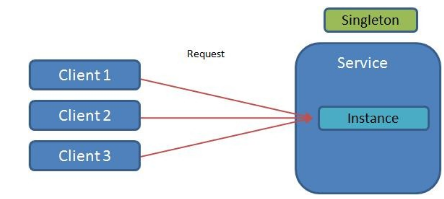
\includegraphics[width=1\linewidth]{images/singleton}
\end{center}
\caption{Singleton}
\label{fig:6}
\end{figure}

\subsubsection{Web service}
 Un service web (ou service de la toile 1) est un protocole d'interface informatique de la famille des technologies web permettant la communication et l'échange de données entre applications et systèmes hétérogènes dans des environnements distribués. Il s'agit donc d'un ensemble de fonctionnalités exposées sur internet ou sur un intranet, par et pour des applications ou machines, sans intervention humaine, de manière synchrone ou asynchrone. Le protocole de communication est défini dans le cadre de la norme SOAP dans la signature du service exposé (WSDL). Actuellement, le protocole de transport est essentiellement HTTP(S).\cite{webservice}


\textbf{Web service REST}

Le World Wide Web est une application conçue selon l'architecture REST. L'architecture du Web remplace donc les concepts applicatifs clients et serveurs par les concepts agents et ressources. Des agents interagissent avec des ressources pour créer, accéder, modifier ou supprimer une ressource. Jusqu'à présent, on parlait surtout de l'interaction entre agents utilisateurs, principalement les navigateurs avec les ressources.

Aujourd'hui, on parle de plus en plus de l'interaction entre agents ressources ; c'est-à-dire la relation entre les ressources : une ressource devient l'agent d'une autre ressource, mais reste elle-même une ressource accessible par d'autres agents. C'est exactement l'architecture décrite par l'exemple d'implémentation applicative des mashups.

Les services web traitent donc d'agents ressources là où le mode opératoire classique du Web parle d'agents utilisateurs. Mais les deux concepts reposent sur la même architecture : REST.
Il n'y a donc pas de différence fondamentale entre l'interaction d'un navigateur avec une ressource et celle d'un Service Web avec une ressource. La principale différence se situe au niveau du format de la représentation des données : HTML pour les navigateurs ou agents utilisateurs, XML ou JSON pour les services web ou agents ressources…

On peut donc définir un service web comme l'implémentation logicielle d'une ressource, identifiée par une URL, et accessible en utilisant les protocoles internet. Les agents s'occupent du contenu, de la représentation de leur état, pas du type de contenu. Il faut donc voir les Services Web comme le moyen de manipuler l'information, et non comme un simple fournisseur de services.


\textbf{TALEND ESB}


L’Enterprise Service Bus, ou ESB, est un ensemble de moyens techniques et organisationnels dont le but est de permettre la communication entre des applications qui, à la base, ne sont pas pensées pour fonctionner ensemble.
 On peut considérer l’ESB comme une nouvelle génération d’EAI (Enterprise Application Integration). La différence majeure avec l’EAI réside dans le fait que l’ESB propose une architecture distribuée décentralisée grâce à l’orchestration de services. Ceux-ci contiennent la logique d’intégration et peuvent être déposés au plus près des applications sources si nécessaire.
Le studio de Talend Open Studio for ESB s’appuie sur le studio de la plateforme unifiée de Talend. Il s’agit donc du même studio, basé sur Eclipse, avec des composants dédiés aux fonctionnalités ESB permettant de gérer la gestion des messages, les services Web, le routage et la transformation des données. Il permet ainsi de développer et de publier des services Web Java, des applications REST et des routes de médiation afin de faire communiquer les applications entre elles.\cite{webservice}
 
\begin{figure}[H]
\begin{center}
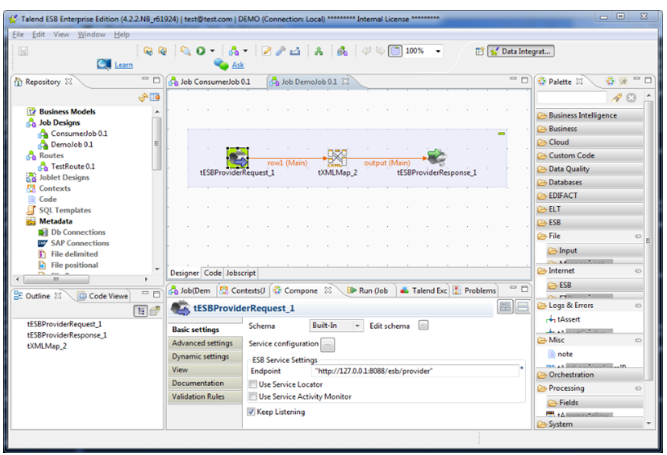
\includegraphics[width=1\linewidth]{images/talend}
\end{center}
\caption{Talend Open Studio for ESB}
\label{fig:7}
\end{figure}

\subsubsection{Crashlytics Fabric}

Crashlytics c’est un outil qui permet de suivre les crashs rencontrés. Concrètement, si une application plante sur l’appareil d’un utilisateur, Crashlytics donne la possibilité d’avoir une trace de ce crash, avec diverses informations comme le nom du téléphone, la version du système d’exploitation, la RAM de libre, l’espace de stockage restant etc. autant d’informations qui peuvent vous aider à cerner la source du problème.

Le dashboard proposé permet de visualiser les crashs par version de l’app, de visualiser le nombre de fois qu’un bug a été rencontré etc.

Cet outil  permet, entre autres, de faire remonter :

- des crashs

- des exceptions

- des messages

- des « customs keys » (pour par exemple connaître l’état de certaines variables)

- des informations sur votre utilisateur.


Renseignez le maximum d’informations permettant de pouvoir cerner la source du problème. \cite{crashlytics} 

\begin{figure}[H]
\begin{center}
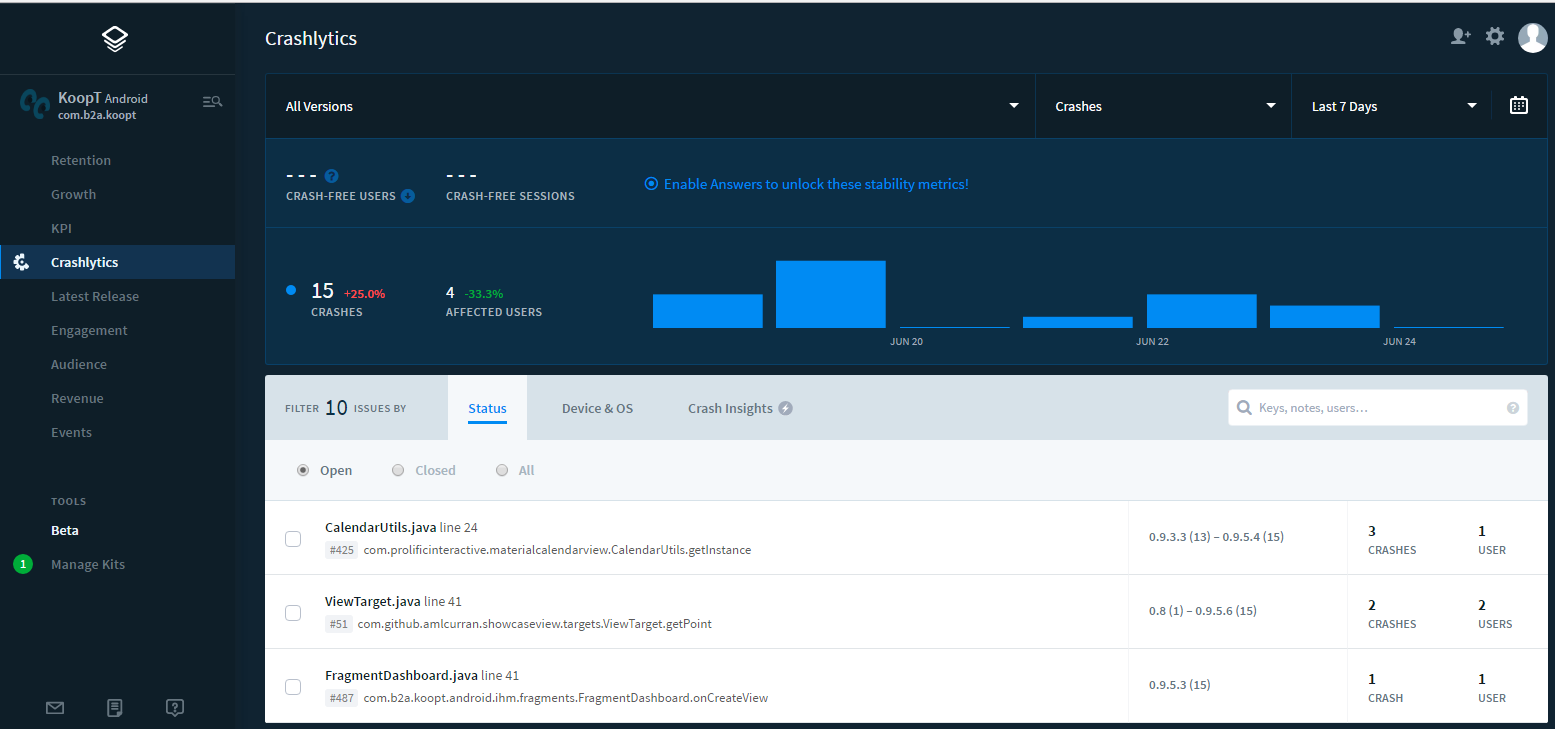
\includegraphics[width=1\linewidth]{images/crashlytics}
\end{center}
\caption{Crashlytics KOOPT}
\end{figure}

\section{Analyse décisionnelle des systèmes complexes}

\subsection{Modélisation des systèmes Complexes}

B-ADSc : "Bucki – Analyse décisionnelle des Systèmes complexes" est une méthode dédiée à la conception et à l’analyse des systèmes et des organisations. Elle se distingue par la prise en compte effective des opérateurs humains avec leurs autonomies, leurs politiques de production, leurs procédés de prise de décision, leur retour d’expérience...

Dans la conception du Système d'Information, les flux des données et des traitements sont soumis aux flux des décisions : en cela B-ADSc généralise les analyses fonctionnelles. Ainsi, le Système d’information est intimement lié à l’Organisation des acteurs (hommes, machines) jusqu'à se confondre.

Conçue dans les années 1990 par Janusz Bucki, docteur en mathématiques et ingénieur automaticien, alors qu’il conduisait des réalisations dans le domaine de l’industrie et de la défense en particulier pour la conception des systèmes à risque et à Intelligence distribuée, cette approche s’est étendue depuis au tertiaire, au monde de l'Internet - Internet des objets - et donne lieu à un enseignement.

Selon cette approche systémique, la caractéristique la plus importante de toute organisation est sa capacité à élaborer des Décisions relatives au pilotage des processus : elle s'attache donc à modéliser et à analyser les organisations selon l'ordonnancement des Décisions et non selon l'agencement des Fonctions...

Pour B-ADSc, une organisation correspond à une hiérarchie opérationnelle d’activités dans laquelle chaque activité représente un «centre élémentaire de prise de décision» pouvant être piloté par un homme ou par une machine.\cite{badsc} 

\begin{figure}[H]
\begin{center}
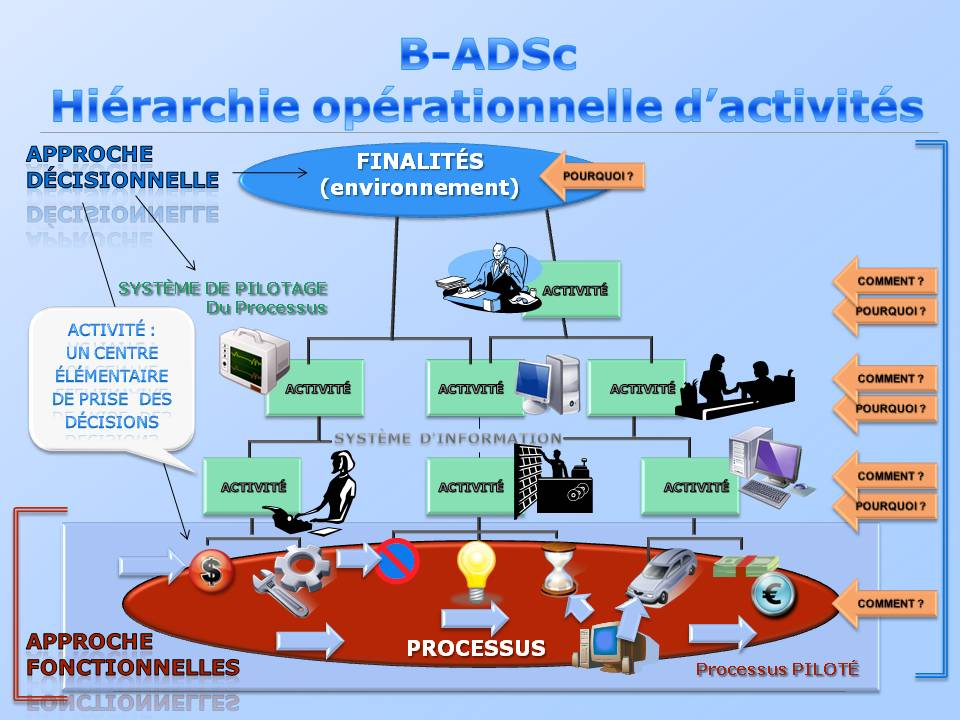
\includegraphics[width=1\linewidth]{images/badsc}
\end{center}
\caption{Hiérarchie opérationnelle d'activités}
\label{fig:8}
\end{figure}


\subsection{ Le concept d’activité}

En Analyse fonctionnelle, l’accent est mis sur les données (schémas de données) et leur transformation ou traitement (schémas des traitements). Ainsi, l’objectif de l’analyste serait plutôt de mettre en exergue le « comment » du système (voir schéma ci-dessous) et pas forcément le « pourquoi de ce comment ».

\begin{figure}[H]
\begin{center}
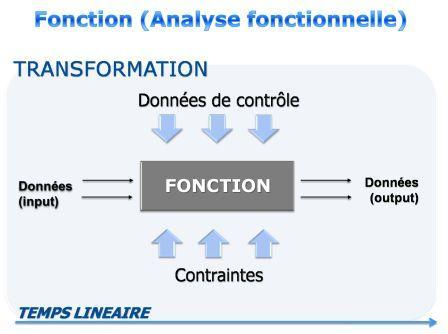
\includegraphics[width=0.5\linewidth]{images/analyse_fonctionnelle}
\end{center}
\caption{L'analyse fonctionnelle}
\label{fig:9}
\end{figure}

Ici, la fonction est comparable à une boîte noire. Elle peut être décomposée en sous-boîtes noires, l'organisation de ces boîtes n'ayant pas pour but de refléter l'organisation des acteurs. En automatisation, la notion de boucle de régulation permet d’adjoindre un « retour » (ou feedback) afin de passer du traitement à la régulation. La fonction peut donc, selon l’évolution du processus, être régulée.

B-ADSc positionne systématiquement le "Comment" dans le contexte de son "Pourquoi" et fait passer du "traitement des données" au "pilotage/régulation des situations" : piloter/gérer un processus signifie décider et contrôler son évolution afin de l’amener à une situation concordant avec les objectifs poursuivis.
La compréhension et l'interprétation des évolutions du processus s’opèrent dans le contexte des buts du décideur, exemple:
Evolution du processus : "je suis chez moi et il commence à pleuvoir"...
si mon but initial est d’arroser le jardin alors - c’est bon – "la nature s’en charge"si mon but est d’aller au théâtre alors - c’est mauvais - "risque d’être mouillé".

Les objectifs et le processus évoluant, le pilotage doit être perpétuellement réadapté : les écarts entre objectifs et réalité doivent diminuer ou, à minima, s’inscrire dans un seuil de tolérance (qui permet d’amener la situation – le processus – au plus près des objectifs poursuivis).
B-ADSc place ici l'activité à l’intersection de deux boucles de régulation qui prennent en compte l’évolution du processus (le comment) et celle des objectifs (le pourquoi).
 
 \begin{figure}[H]
\begin{center}
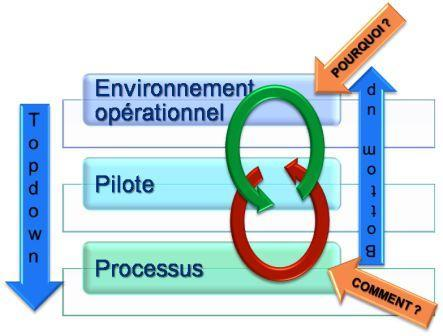
\includegraphics[width=0.5\linewidth]{images/comment_pourquoi}
\end{center}
\caption{L'intersection des deux boucles de régulation le comment et le pourquoi}
\label{fig:10}
\end{figure}
La « brique » de base de B-ADSc est une Activité. Elle est régulée (ou pilotée) par les activités de niveau supérieur qui lui délèguent des objectifs et régule (ou pilote) les activités de niveau inférieur qui constituent son processus.
Ainsi, elle encapsule deux fonctions
(voir schéma ci-dessous):

• « Fd » pour « Fonction décision » 

• « Fe » pour « Fonction évaluation » 

Une activité dispose nécessairement de quatre mémoires distinctes :

1.La mémoire des objectifs assignés par le niveau opérationnel supérieur 

2.La mémoire de l'état du processus piloté 

3.La mémoire des buts des décisions prises par l’activité 

4.La mémoire des changements d’état du processus

 
 \begin{figure}[H]
\begin{center}
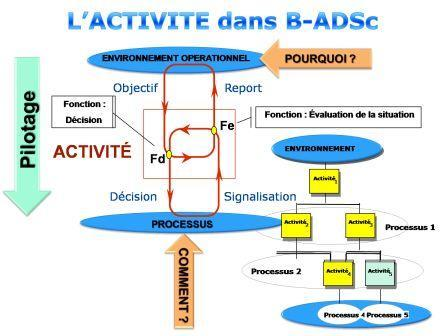
\includegraphics[width=1\linewidth]{images/activite}
\end{center}
\caption{L'activité dans B-ADSc}
\label{fig:11}
\end{figure}

 
B-ADSc interprète systématiquement le comportement d’une activité – prise des décisions, évaluation du processus - dans le contexte des objectifs poursuivis :
Je suis chez moi (« Je » = activité) et il pleut dehors (le « comment » du processus).

• Si mon but initial est d’arroser le jardin alors « c’est bon pour moi » (la nature fera à ma place, je n'ai rien à décider sauf annuler l'arrosage) 

• Si mon but est d’aller au théâtre alors « c’est mauvais pour moi » (je risque d’y arriver mouillé, je décide donc d'annuler ou de prendre un parapluie).\cite{badsc} 


\subsubsection{Caractéristique}

La tolérance et la sensibilité font partie des caractéristiques comportementales d’une activité pilotée.
 
- Tolérance : exprime l’écart maximum admissible pour l'activité pilotée entre l'état perçu du
processus (état interne) et l'objectif poursuivi (objectif externe).
 
- Sensibilité : correspond aux évolutions du processus jugées significatives dans le contexte de
l’un des buts (objectifs internes) de l’activité.
 
Tolérance et sensibilité, peuvent être :
 
• prescrites : imposées de façon structurelle

• conjoncturelles : corrigées (consciemment ou inconsciemment) par le pilote de l’activité
 
Lorsque les objectifs sont validés par le niveau opérationnel supérieur et que les procédures de mise en œuvre des savoirs sont imposées, l’autonomie d’une activité ou d’un acteur et, par là même, sa politique locale de production ou de pilotage ne pourront s’exprimer qu’à travers la tolérance et la sensibilité conjoncturelle.
 
Dans une activité de 1e catégorie il s'agit de la seule forme d’expression de son autonomie.
Dans une activité de 2e catégorie, la politique locale intègre en plus l’expression des préférences
face aux sollicitations simultanées – Fp.
Dans une activité de 3e catégorie, la politique locale comprendra en plus les conditions d’auto
validation des objectifs (externes). \cite{activite}

\subsection{Avantage}

La délégation des décisions, selon la méthode B-ADSc, est par excellence le facteur structurant des organisations. Les délégations conduisent à l’émergence d'activités nouvelles pilotées par des hommes ou par des machines, chacune d’elles constituant un centre autonome de prise des décisions. Pour être efficaces, de telles délégations doivent s’accompagner de la délégation des contrôles correspondants. 

Le rôle de l’activité « déléguant » évolue pour devenir tributaire de décisions de portée plus générale. Suite à une délégation, le nombre de décisions à prendre dans une organisation augmente globalement, tout comme l’effort à fournir pour leur élaboration.
La délégation des décisions peut aussi bien être liée à la création d'activités nouvelles et à l'extension du système d’information.
Compte tenu du coût qui en résulte, toute nouvelle délégation requiert pour sa validation une analyse de la valeur.

Cette analyse, conduite pour évaluer les gains potentiels, suit trois axes :

• amélioration du fonctionnement 
  - décisions plus pertinentes élaborées au niveau du système de délégation : suppression d’une non qualité, 
  
• augmentation de la productivité 
  - par une diminution du délai de prise de décision par rapport au rythme de déroulement du processus : davantage de volumes traités, 
  
• disponibilité accrue des acteurs opérant dans les couches supérieures 
  - grâce à la substitution des décisions déléguées par des décisions plus globales et moins fréquentes: dégageant un potentiel pouvant être réemployé par ailleurs. \cite{badsc}
 
\subsection{Utilisations}

 B-ADSc s'applique à :

- La Conception et l'Analyse des Systèmes et des Organisations	

- La Démarche qualité, la mise en oeuvre des politiques de veille et innovation

- L'Urbanisation en informatique 

- L'Ingénierie des connaissances (gestion des connaissances) et Gestion du retour d’expérience 

- La Conception des Systèmes d’automatisation et des Systèmes Informatiques 

- L'Explicitation des politiques de production et construction de la "convergence des buts" au sein des organisations

- La Robotique 

- Les Systèmes à Intelligence distribuée ou répartie, les Systèmes experts 1 - notamment pour l'Internet des Objets

- Plus généralement : tout Système critique (transports, aviation, systèmes embarqués, …) 
 
 
\textbf{Thin-Track}, moteur évolutif de gestion des actifs ou objets en environnements industriels ou logistiques changeants et incertains, est la réalisation la plus récente de l'utilisation de B-ADSc, tant en conception logicielle qu'en gestion de projet. \cite{badsc}

\subsection{Modélisation des processus dans KOOPT}

Pourquoi la modélisation des processus dans les projets d'organisation ?
pour administrer les processus et les optimiser : 

    • optimiser les coûts internes,
    
    • améliorer sa réactivité et sa rapidité,
    
    • capitaliser ses propres savoirs et expériences,
    
    • identifier et valider les besoins en information de chaque acteur et chaque activité,
    
    • évaluer les opportunités en délégation/automatisation,
    
    • séparer et structurer les rôles et les responsabilités de chacun des acteurs, homme ou machine,
    
    • concevoir les solutions informatisées s'inscrivant naturellement dans la continuité des chaînes
      décisionnelles propres à l’organisation qui les intègre,
    
    • former les nouveaux arrivants,
    
    • gérer efficacement les adaptations aux nouvelles exigences et aux évolutions du contexte opérationnel.
     
     
pour représenter le processus tel qu'il est vécu et tel qu'il évolue : 
Cette nécessaire modélisation des processus implique une mise en évidence de l'organisation réelle.
Il s'agit non de décrire le processus tel qu'il est défini, mais tel qu'il est réellement vécu.
La modélisation sera donc jugée par sa clarté et sa cohérence dans l’explicitation :

    • des objectifs poursuivis à chaque niveau opérationnel,
    
    • des procédés associés à ces objectifs, donc des ordonnancements des décisions,
    
    • de l'utilité des ressources sollicitées durant la mise en œuvre de ces procédés.

\subsubsection{DOMIS}


La modélisation du KOOPT est réalisée par l’outil : DOMIS
DoMIS permet de documenter les processus dans une entreprise ou dans une administration, quelle que soit leur nature.

Il propose un langage générique fondé sur une vision renouvelée de l’organisation.
Une organisation correspond ici à une hiérarchie opérationnelle d’activités dans laquelle chaque activité représente un « centre élémentaire de prise des décisions » pouvant être piloté par un homme ou une machine.
DoMIS à vocation à modéliser les processus par la mise en évidence du système réel de délégation propre à l'organisation. 

Par différence avec les approches classiques et une analyse statique du déroulement des processus – fonctions, 
DoMIS propose une analyse dynamique du système de pilotage et de ses capacités à décider et agir.
L’expression du pilotage sous forme d’ordonnancement des décisions prévaut ici sur la description du déroulement de la fonction :

• « comment nous le faisons » plutôt que « comment ça doit se faire ».

• DoMIS facilite l'identification d'indicateurs internes de gestion plus opérationnels que ceux quantifiant 
simplement les résultats intermédiaires ou finaux. \cite{domis}



%%% Local Variables: 
%%% mode: latex
%%% TeX-master: "isae-report-template"
%%% End: 